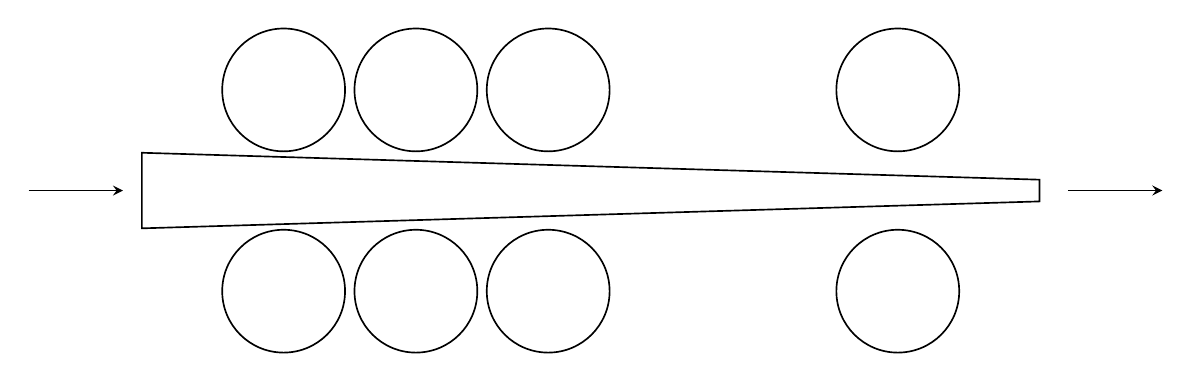
\begin{tikzpicture}[scale=1.2, >=stealth]
    % 1. 绘制中间的带钢 (从左向右逐渐变薄)
    % 左端点 x=0，右端点 x=9.5
    % 经过精确计算斜率，使其刚好与下方的轧辊相切
    \draw[semithick] (0, 0.4) -- (9.5, 0.115) -- (9.5, -0.115) -- (0, -0.4) -- cycle;

    % 2. 绘制上排轧辊 (4个圆)
    % fill=white 能够遮盖掉圆内部的带钢线条，完美还原原图效果
    \draw[semithick, fill=white] (1.5, 1.065) circle (0.65);
    \draw[semithick, fill=white] (2.9, 1.065) circle (0.65);
    \draw[semithick, fill=white] (4.3, 1.065) circle (0.65);
    \draw[semithick, fill=white] (8.0, 1.065) circle (0.65);

    % 3. 绘制下排轧辊 (4个圆，纵坐标与上排对称)
    \draw[semithick, fill=white] (1.5, -1.065) circle (0.65);
    \draw[semithick, fill=white] (2.9, -1.065) circle (0.65);
    \draw[semithick, fill=white] (4.3, -1.065) circle (0.65);
    \draw[semithick, fill=white] (8.0, -1.065) circle (0.65);

    % 4. 绘制输入与输出的指示箭头
    \draw[->, semithick] (-1.2, 0) -- (-0.2, 0);
    \draw[->, semithick] (9.8, 0) -- (10.8, 0);

\end{tikzpicture}